% --------------------------------------------------------------------------- %
% Poster for the ECCS 2011 Conference about Elementary Dynamic Networks.      %
% --------------------------------------------------------------------------- %
% Created with Brian Amberg's LaTeX Poster Template. Please refer for the     %
% attached README.md file for the details how to compile with `pdflatex`.     %
% --------------------------------------------------------------------------- %
% $LastChangedDate:: 2011-09-11 10:57:12 +0200 (V, 11 szept. 2011)          $ %
% $LastChangedRevision:: 128                                                $ %
% $LastChangedBy:: rlegendi                                                 $ %
% $Id:: poster.tex 128 2011-09-11 08:57:12Z rlegendi                        $ %
% --------------------------------------------------------------------------- %
\documentclass[a0paper,portrait]{baposter}

\usepackage{subfigure}
\usepackage{amsmath}	
\usepackage{relsize}		% For \smaller
\usepackage{url}			% For \url
\usepackage{multirow} % For \multirow and \multicolumn in tables
\usepackage[export]{adjustbox}
\usepackage{caption}
\usepackage{ragged2e}
\usepackage{siunitx}
% \usepackage{epstopdf}	% Included EPS files automatically converted to PDF to include with pdflatex

%%% Global Settings %%%%%%%%%%%%%%%%%%%%%%%%%%%%%%%%%%%%%%%%%%%%%%%%%%%%%%%%%%%

\graphicspath{{Figures/}}	% Root directory of the pictures 
% \tracingstats=2			% Enabled LaTeX logging with conditionals

%%% Color Definitions %%%%%%%%%%%%%%%%%%%%%%%%%%%%%%%%%%%%%%%%%%%%%%%%%%%%%%%%%

\definecolor{bordercol}{RGB}{80,80,180}
\definecolor{headercol1}{RGB}{186,215,230}
\definecolor{headercol2}{RGB}{80,80,180}
\definecolor{headerfontcol}{RGB}{0,0,0}
%\definecolor{boxcolor}{RGB}{186,215,230}
\definecolor{boxcolor}{RGB}{255,255,255}

%%%%%%%%%%%%%%%%%%%%%%%%%%%%%%%%%%%%%%%%%%%%%%%%%%%%%%%%%%%%%%%%%%%%%%%%%%%%%%%%
%%% Utility functions %%%%%%%%%%%%%%%%%%%%%%%%%%%%%%%%%%%%%%%%%%%%%%%%%%%%%%%%%%

%%% Save space in lists. Use this after the opening of the list %%%%%%%%%%%%%%%%
\newcommand{\compresslist}{
	\setlength{\itemsep}{1pt}
	\setlength{\parskip}{0pt}
	\setlength{\parsep}{0pt}
}

\newcommand\pro{\item[$+$]}
\newcommand\con{\item[$-$]}

\newenvironment{packed_itemize}{
	\begin{itemize}
		\setlength{\itemsep}{1pt}
		\setlength{\parskip}{0pt}
		\setlength{\parsep}{0pt}
	}{\end{itemize}}
%%%%%%%%%%%%%%%%%%%%%%%%%%%%%%%%%%%%%%%%%%%%%%%%%%%%%%%%%%%%%%%%%%%%%%%%%%%%%%%
%%% Document Start %%%%%%%%%%%%%%%%%%%%%%%%%%%%%%%%%%%%%%%%%%%%%%%%%%%%%%%%%%%%
%%%%%%%%%%%%%%%%%%%%%%%%%%%%%%%%%%%%%%%%%%%%%%%%%%%%%%%%%%%%%%%%%%%%%%%%%%%%%%%

\begin{document}
	\typeout{Poster rendering started}
	
	%%% Setting Background Image %%%%%%%%%%%%%%%%%%%%%%%%%%%%%%%%%%%%%%%%%%%%%%%%%%
	\background{
		\begin{tikzpicture}[remember picture,overlay]%
		\draw (current page.north west)+(-2em,2em) node[anchor=north west]
		{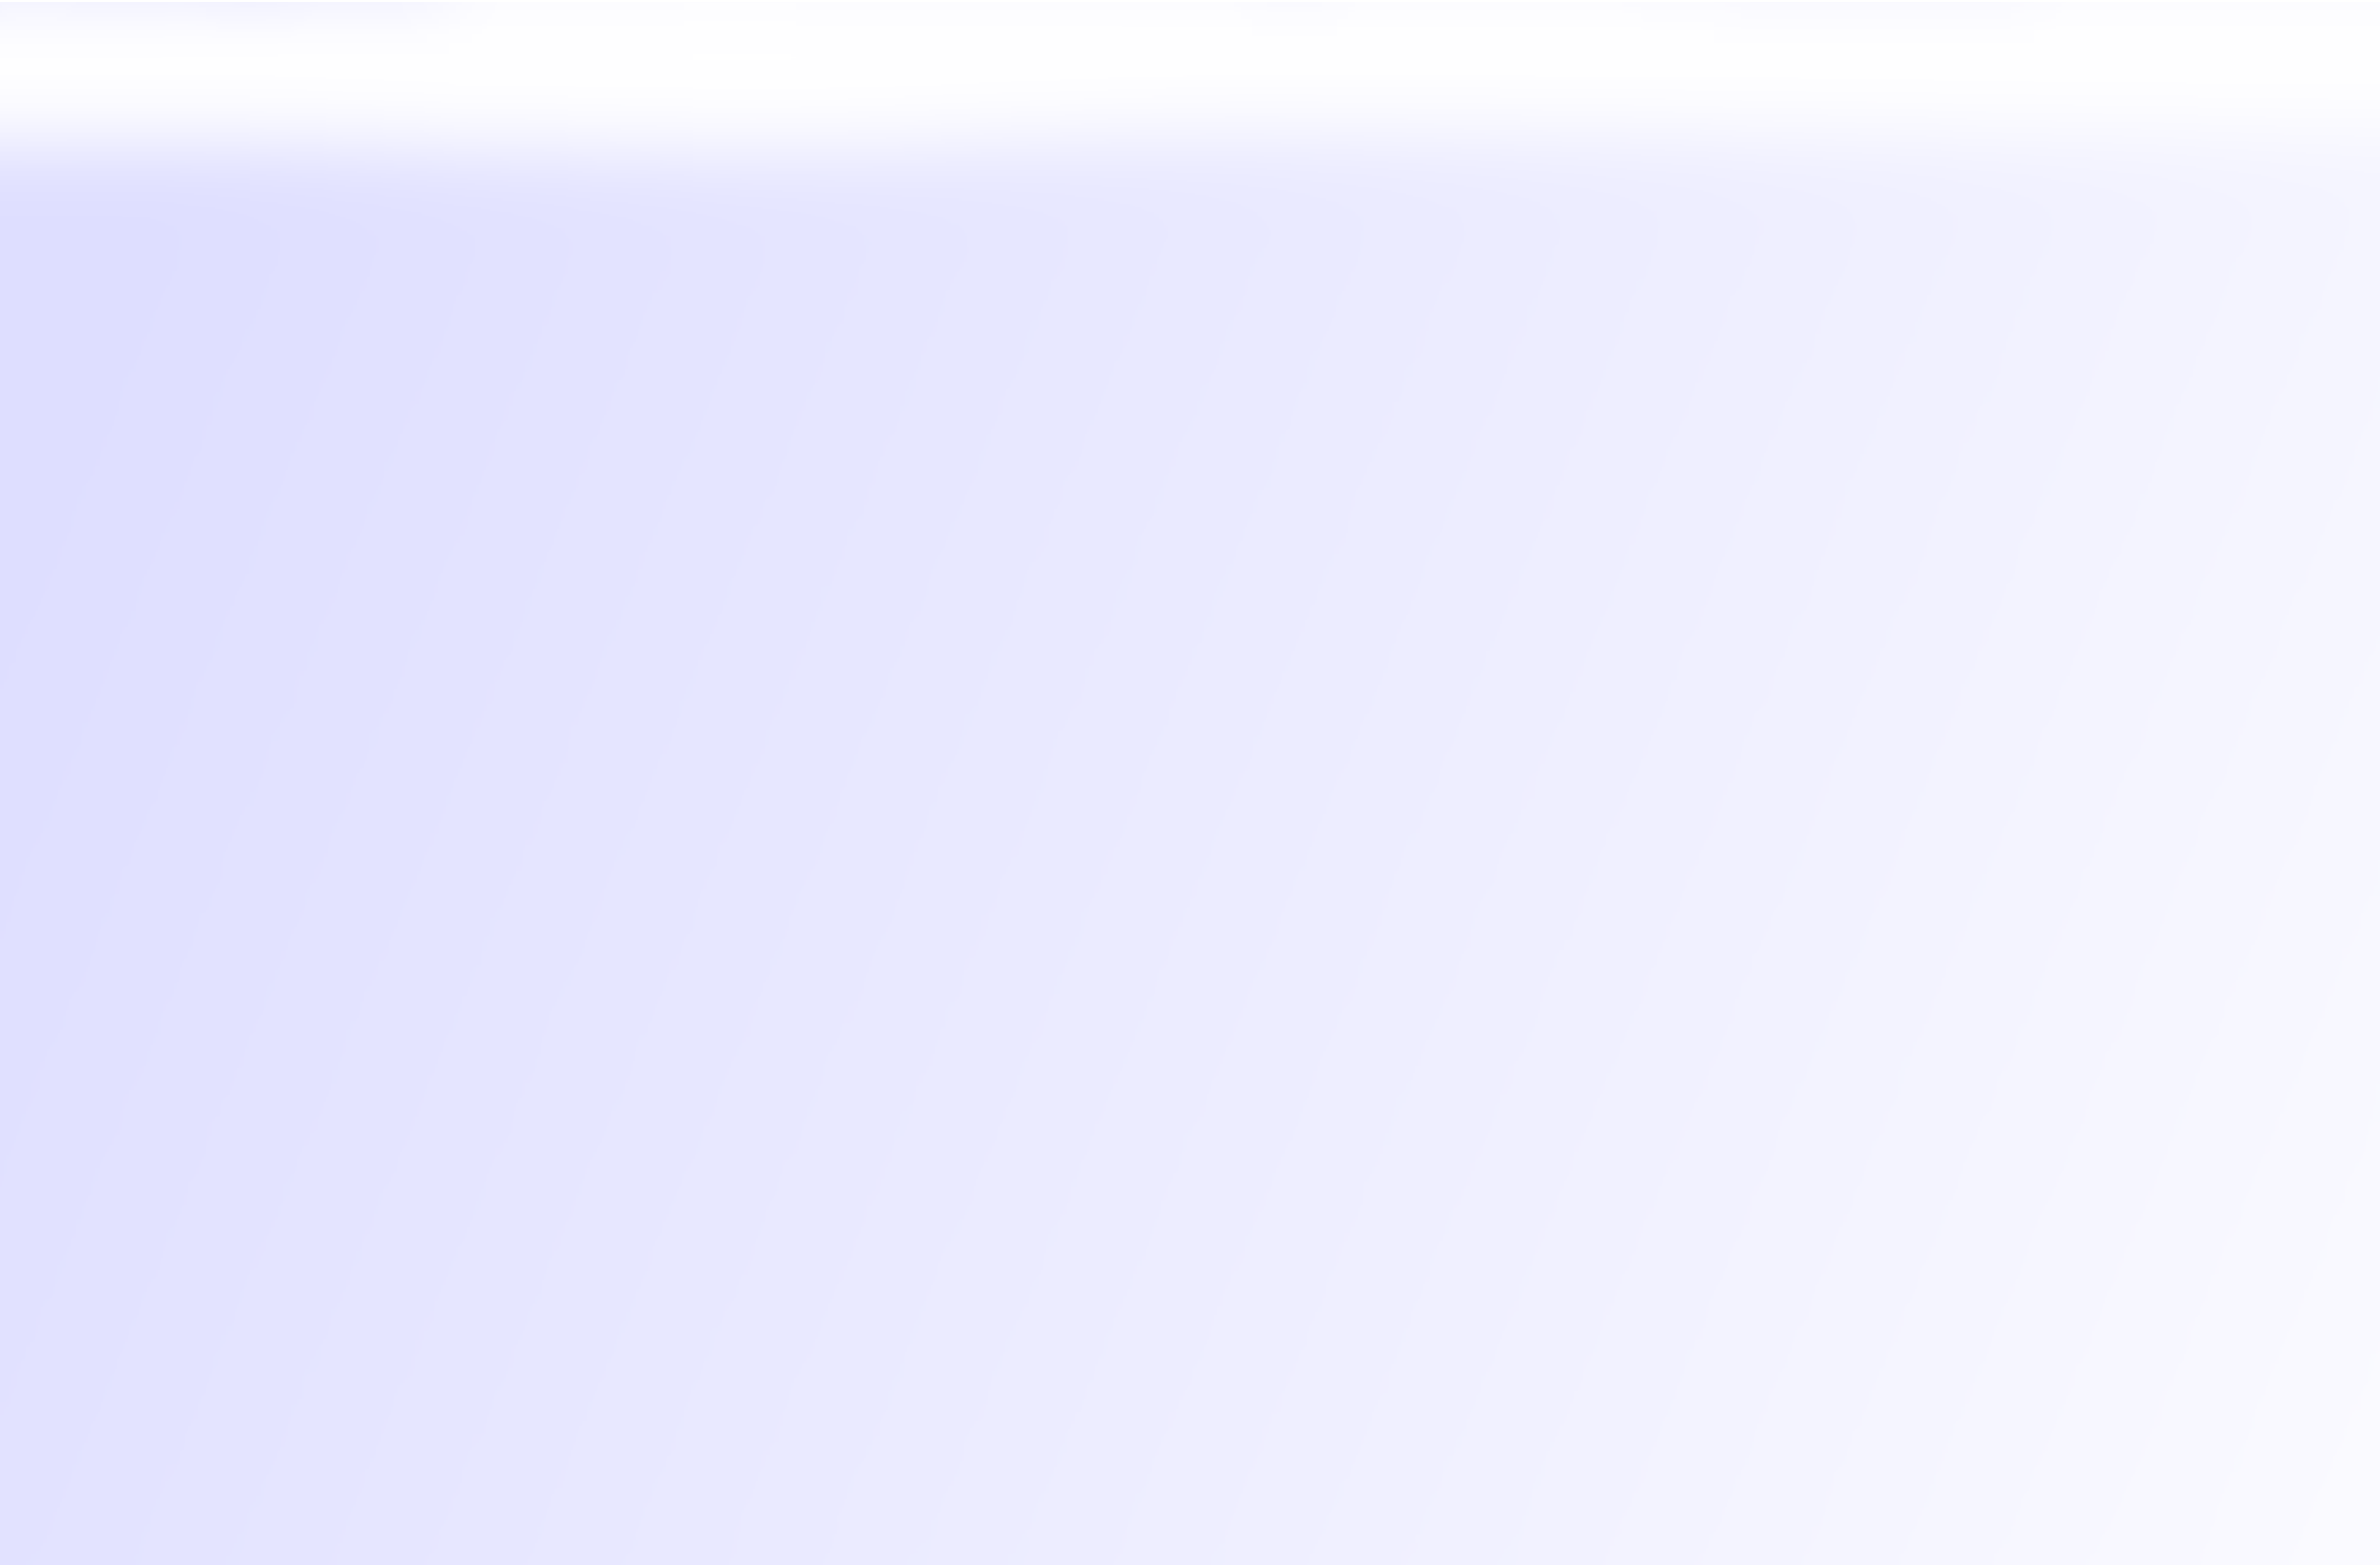
\includegraphics[height=1.1\textheight]{./Figures/background}};
		\end{tikzpicture}
	}
	
	%%% General Poster Settings %%%%%%%%%%%%%%%%%%%%%%%%%%%%%%%%%%%%%%%%%%%%%%%%%%%
	%%%%%% Eye Catcher, Title, Authors and University Images %%%%%%%%%%%%%%%%%%%%%%
	\begin{poster}{
		    %general options for the poster
			grid=false,
			columns=3, % how many columns 1-6
			colspacing=4.2mm, % spacing between the columns
			headerheight=0.15\textheight, % the height of the header as a proportion of the page height
			background=user, %user or none or plain
			eyecatcher=true, %turn logos on/off
			% Option is left on true though the eyecatcher is not used. The reason is
			% that we have a bit nicer looking title and author formatting in the headercol
			% this way
			borderColor=bordercol, %darkgray,
			headerColorOne=headercol1, %darkgray,
			headerColorTwo=headercol2,
			headerFontColor=headerfontcol,
%			headerborder=open,
			headerborder=closed, % see the baposter manual for the rest
			headershape=roundedright, %rectangle,
			%headershade=plain,
			%headerFontColor=white,
%			headerfont=\large\bfseries,
			headerfont=\Large\sf\bf,
			%posterbox options
			textborder=rectangle,
			boxshade=plain,
			% Only simple background color used, no shading, so boxColorTwo isn't necessary
			boxColorOne=boxcolor, %white,
			linewidth=1pt
		}
		%%% Eye Cacther (or left side logo's) %%%%%%%%%%%%%%%%%%%%%%%%%%%%%%%%%%%%%%%%%
		{
			\setlength{\tabcolsep}{2pt}
			\begin{tabular}{cc}
				
\includegraphics[height=6em]{DEFENCE-LogoColor-TextBlack-print} & 
\includegraphics[height=6em]{logo_irsd} \\
				\multicolumn{2} {c} {
\includegraphics[height=6em]{Logo_RMA}}
			\end{tabular}
		}
		%%% Title %%%%%%%%%%%%%%%%%%%%%%%%%%%%%%%%%%%%%%%%%%%%%%%%%%%%%%%%%%%%%%%%%%%%%
		{High-fidelity numerical simulations on airfoils at low-Reynolds number}
		%%% Authors %%%%%%%%%%%%%%%%%%%%%%%%%%%%%%%%%%%%%%%%%%%%%%%%%%%%%%%%%%%%%%%%%%%
		{
			\vspace{0.7cm} C. Brunelli $^{1,2,3}$, B. Janssens $^1$, B. Marinus $^1$, G. May $^2$, M. Runacres $^3$\\
			{
				\footnotesize $^1$ Royal Military Academy, Department of Mechanical Engineering, Brussels, Belgium \\
				$^2$ Von Karman Institute for Fluid Dynamics, Sint-Genesius-Rode, 1640, Belgium  \\
				$^3$ Vrije Universiteit Brussel, Brussels, Belgium  \\
				\textbf{carlo.brunelli@mil.be} }
		}
		%% Right's side logo's %%%%%%%%%%%%%%%%%%%%%%%%%%%%%%%%%%%%%%%%%%%%%%%%%%%%%%%%
		{
				%\setlength{\tabcolsep}{2pt}
				\renewcommand{\arraystretch}{3}
				\begin{tabular}{ccc}
				   
\includegraphics[height=3em]{vki_nobg}\\
					\multicolumn{1} {c} {
\includegraphics[height=3.7em]{VUB_nobg}}\\
					\multicolumn{1} {c}
					{
\includegraphics[height=3em]{NELSHAW}}
				\end{tabular}
		}


\headerbox{Research Purpose}{name=purpose,column=0,span=3,row=0}{
		\begin{minipage}{0.65\textwidth}
		The request for numeric models for transitional airfoils has grown in the recent years thanks to their emerging applications for high-altitude pseudo-satellites (HAPS). Developing new suitable numerical methods avoids expensive and time-consuming experimental testing and helps to identify promising geometries. For this purpose, the research has developed a new version of the Variational MultiScale method (VMS) - firstly introduced by \citeauthor{Hughes2005} \cite{Hughes2005} - which belongs to the family of implicit Large Eddy Simulation (iLES).
        
	The project ambitiously aims to extend the capability to solve the adjoint problem - leveraging Automatic Differentiation (AD) - to generate airfoils with better performances.	
		\end{minipage}	
	\hspace{0.01\textwidth}	
		\begin{minipage}{0.3\textwidth}
			\centering
			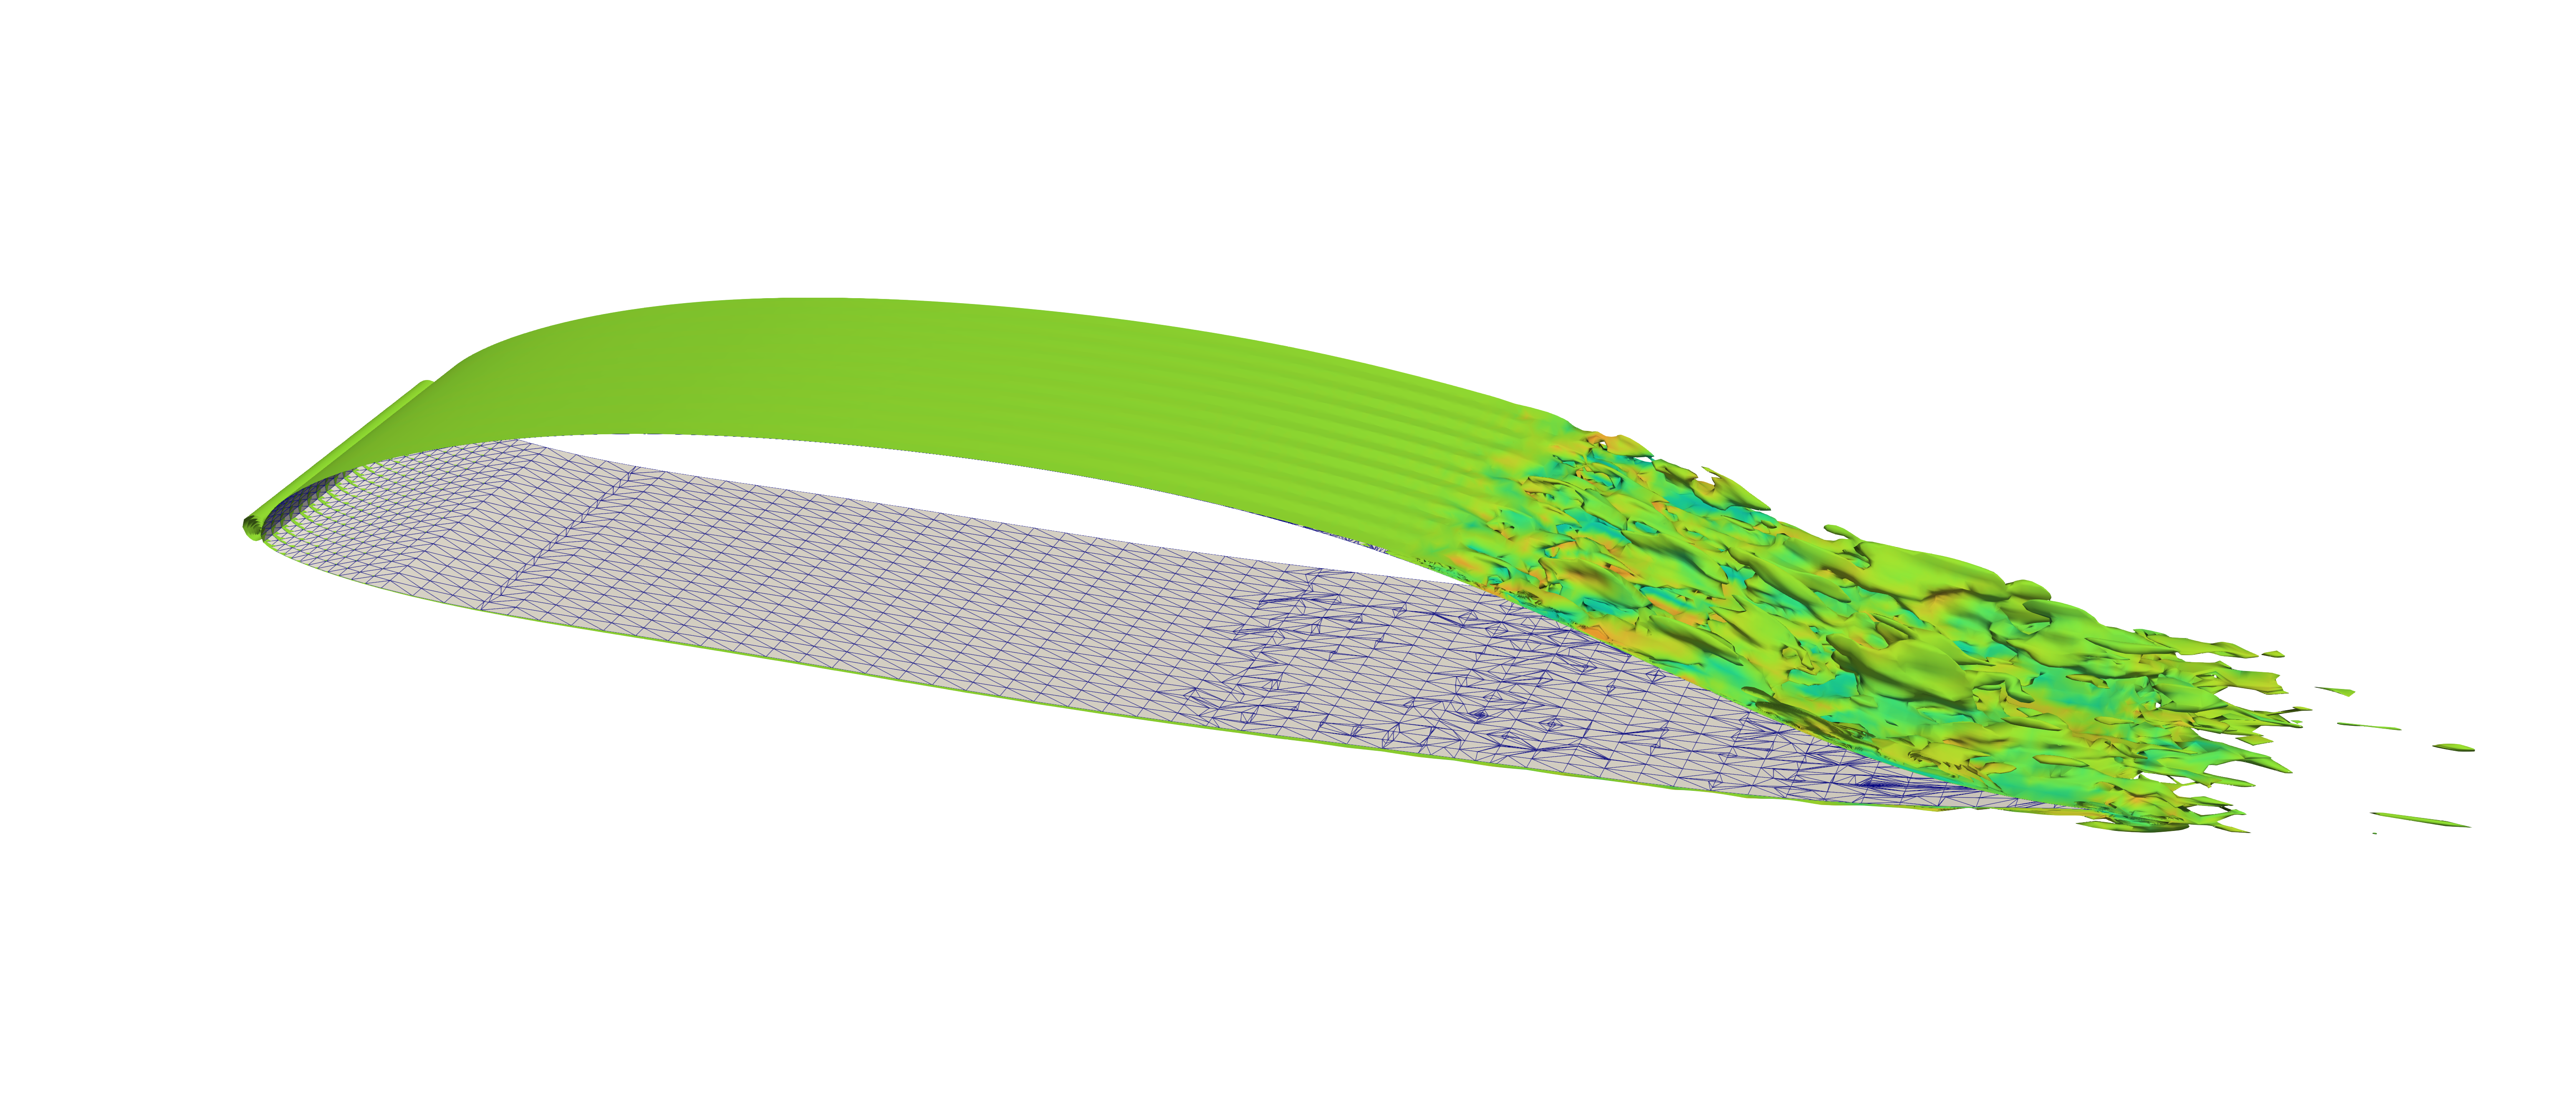
\includegraphics[width= 1\textwidth]{Figures/du89_vcontour.png}
			\begin{minipage}{0.95\textwidth}
			\vspace{0.3 cm}
			\justifying
			\noindent
			\scriptsize \textit{DU89-134 airfoil at Reynolds $\num{500000}$ $\ang{1}$, velocity contour, $u_z$ colormap}
			\end{minipage}
		\end{minipage}	
}

\headerbox{Low Reynolds regime}{name=lowreynolds,column=0,span=1,row=0, below=purpose}{
		\begin{minipage}{0.95\textwidth}
    HAPS flight conditions:
   \begin{packed_itemize}
				\con High altitude: $16-20km$
				\con Low-speed: $Mach\approx 0.1$
				\con Low-Reynolds: $Re\leq500000$
		\end{packed_itemize}
    Developing new suitable numerical methods avoids expensive and time-consuming experimental tests and helps identify promising geometries. The challenges addressed are:
       \begin{packed_itemize}
				\con formation of the Laminar Separation Bubble (LSB)
				\con laminar to turbulent transition
				\con Turbulence Intensity (TI) effects
		\end{packed_itemize}
  			
		\end{minipage}						
}

 
\headerbox{\smaller Variational MultiScale Method}{name=method,span=1,column=0,row=0,below=lowreynolds}{
  A Linearized and Segregated VMS (LS-VMS) has been implemented:
             \begin{packed_itemize}
				\con coded in the Julia programming language
                \con implicit Large Eddy Simulation (iLES)
				\con fully 3-dimensional unsteady 
                \con parallelized 
                \con no calibration needed
		\end{packed_itemize}			
	}
 
\headerbox{Synthetic Eddy Method}{name=sem,span=1,column=0,row=0,below=method}{
It produces realistic and coherent turbulent fluctuations, which deeply influence the transition and separation point. It has also been implemented in Julia \cite{Brunelli2023}. Random fluctuations do not produce a realistic flow, and they are quickly dissipated.			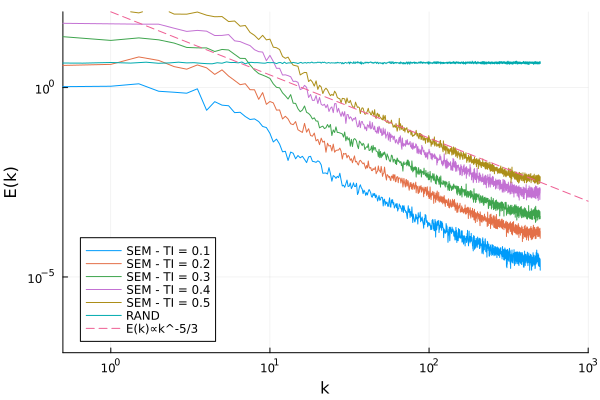
\includegraphics[width= 1\textwidth]{Figures/SEM_vs_RAND_step.png}	
\begin{minipage}{0.95\textwidth}
			\vspace{0.3 cm}
			\justifying
			\noindent
			\scriptsize \textit{Flowfields energy spectra produced using SEM at different turbulence intensity. Comparison with the random generated fluctuations}
\end{minipage}
}

\headerbox{}{name=video,span=1,column=0,row=0, below=sem}{
\begin{minipage}{0.55\textwidth}
Watch a video of an unsteady simulation on YouTube:
\end{minipage}
\begin{minipage}{0.35\textwidth}
\begin{flushright}
    			
\includegraphics[width=0.5\textwidth]{Figures/QRVideo.png}	

\end{flushright}
\end{minipage}
}


\headerbox{Laminar Separation Bubble}{name=lsb ,span=1,column=1,row=0, below=purpose}{
LS-VMS is able to capture the LSB on transitional airfoils. The RANS method, implemented in STARCCM +, uses the transitional model $\gamma-Re_\theta$ which is based on a series of experimental correlations; see \cite{Schubauer47}. The VMS does not need any previous calibration, experiments, or coefficients to be adjusted. 
  \hspace{0.01\textwidth}	
			\centering
			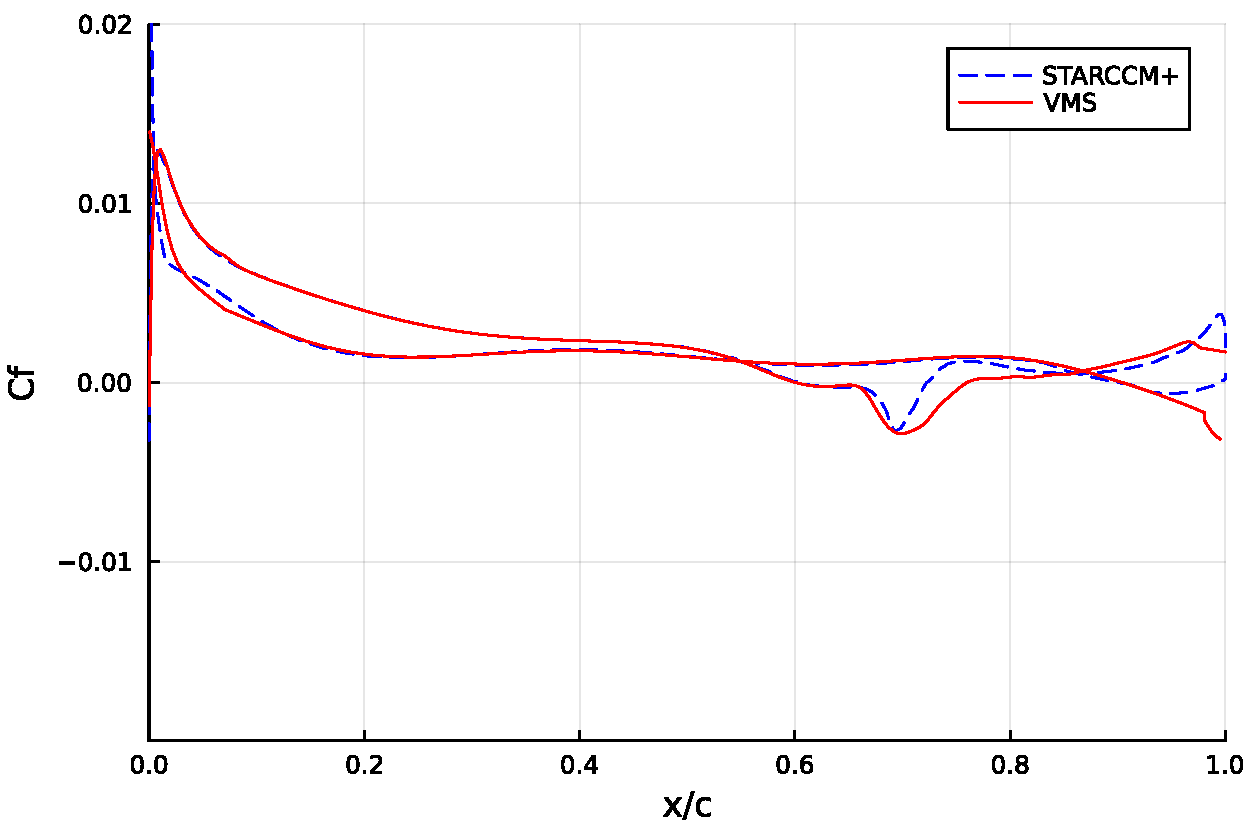
\includegraphics[width= 1\textwidth]{Figures/Freestream_DU89_500000_AoA_1_Cf.pdf}
    		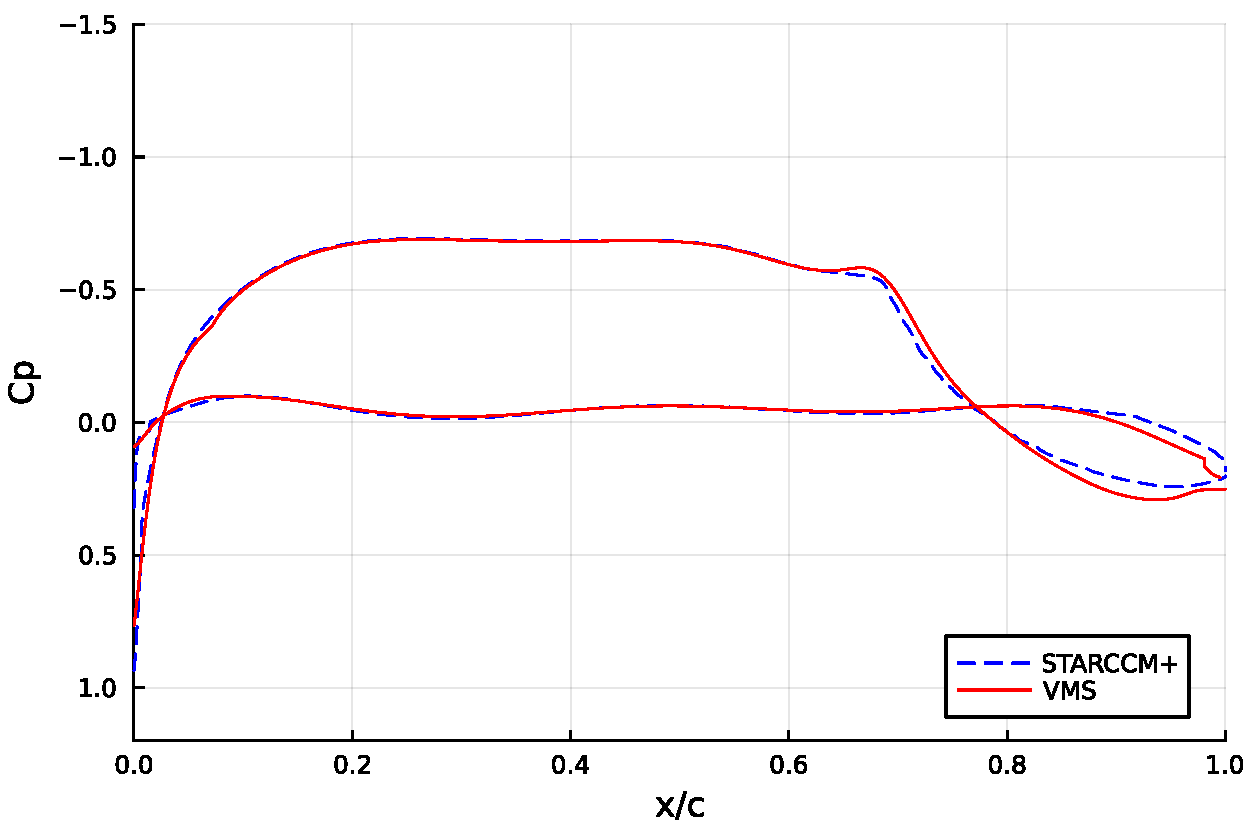
\includegraphics[width= 1\textwidth]{Figures/Freestream_DU89_500000_AoA_1_Cp.pdf}
			\begin{minipage}{0.95\textwidth}
			\vspace{0.1 cm}
			\justifying
			\noindent
			\scriptsize \textit{DU89-134 airfoil at Reynolds $\num{500000}$ $\ang{1}$ pressure and friction coefficient, RANS and LS-VMS comparison}
        \end{minipage}
  	}		

\headerbox{Boundary Layer Initialization}{name=bl_init,span=1,column=1,row=0, below=lsb}{
Avoiding high velocity in small cells of the boundary layer in the initial iterations is crucial to avoid instability. Computing the wall distance and then initializing the boundary layer with a quadratic function ensures numerical stability. 
 \hspace{0.01\textwidth}	
			\centering
			\includegraphics[width= 0.95\textwidth]{Figures/WallDistanceDU89.png}
			\begin{minipage}{0.95\textwidth}
			\vspace{0.1 cm}
			\justifying
			\noindent
			\scriptsize \textit{Velocity magnitude initialization for DU89-134 airfoil}
        \end{minipage}
}	

\headerbox{LSB and Turbulence Intensity}{name=lsb2,span=1,column=2,row=0, below=purpose}{
LSB is deeply affected by free-stream TI. This parameter can be used as an independent variable to tune the results and better match them with experiments.

  \hspace{0.01\textwidth}	
			\centering
			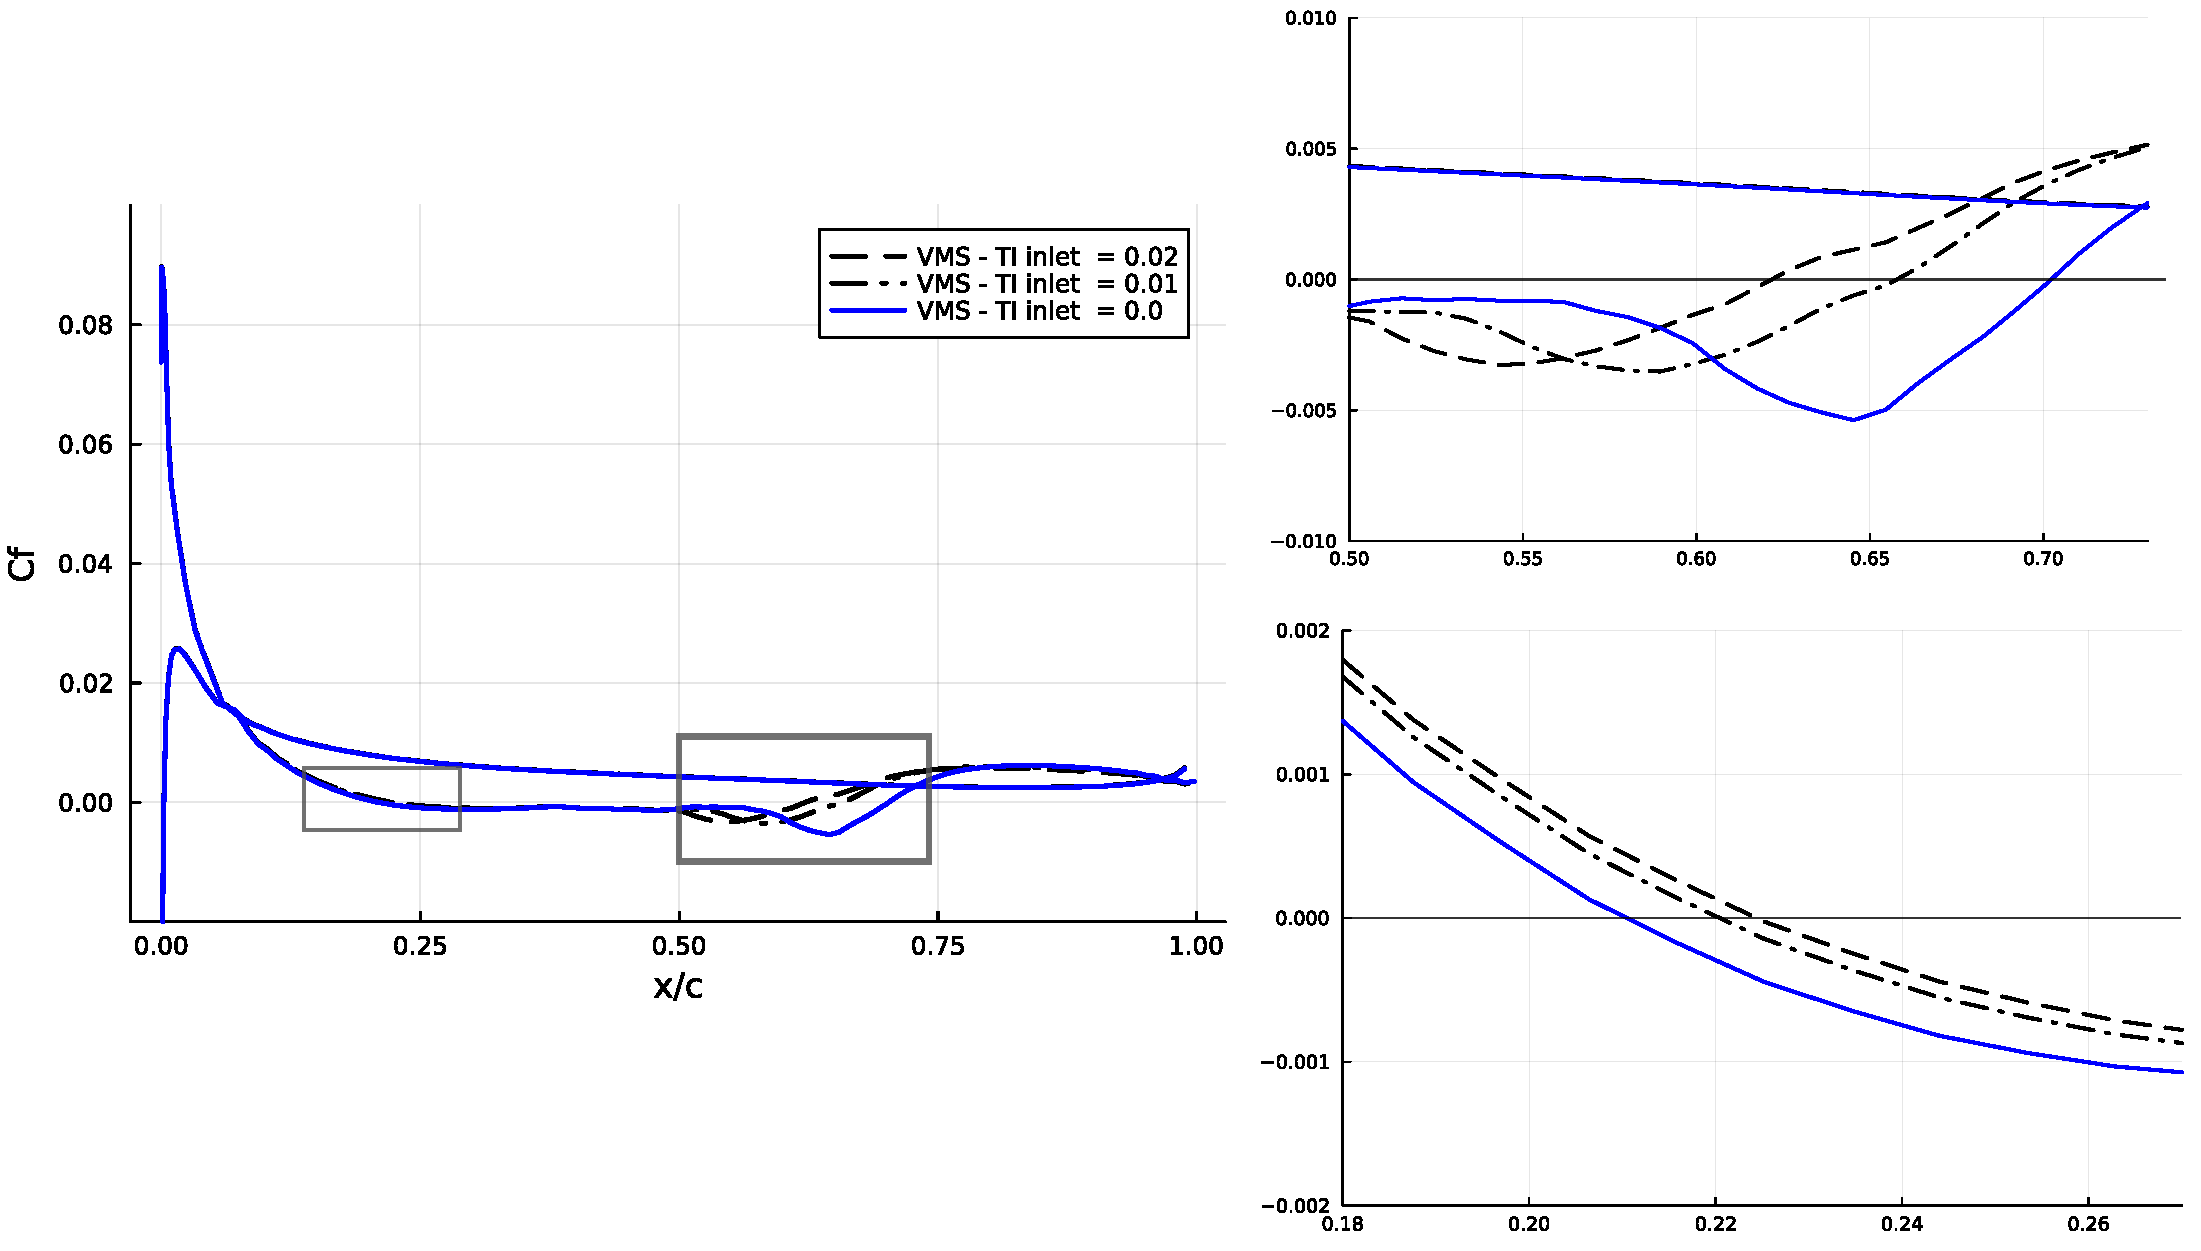
\includegraphics[width= 1\textwidth]{Figures/SD7003_Cf_zoom.pdf}
			\begin{minipage}{0.95\textwidth}
			\vspace{0.1 cm}
			\justifying
			\noindent
			\scriptsize \textit{Friction coefficients at different TI for SD7003 airfoil at Reynolds $\num{60000}$ at $\ang{4}$}
        \end{minipage}
}	   

\headerbox{Uncertainty Quantification}{name=uq,span=1,column=2,row=0, below=lsb2}{
UQ is used to assess the confidence interval of CFD results and identify the closure parameters that most influence the solution.
  \hspace{0.01\textwidth}	
			\centering
			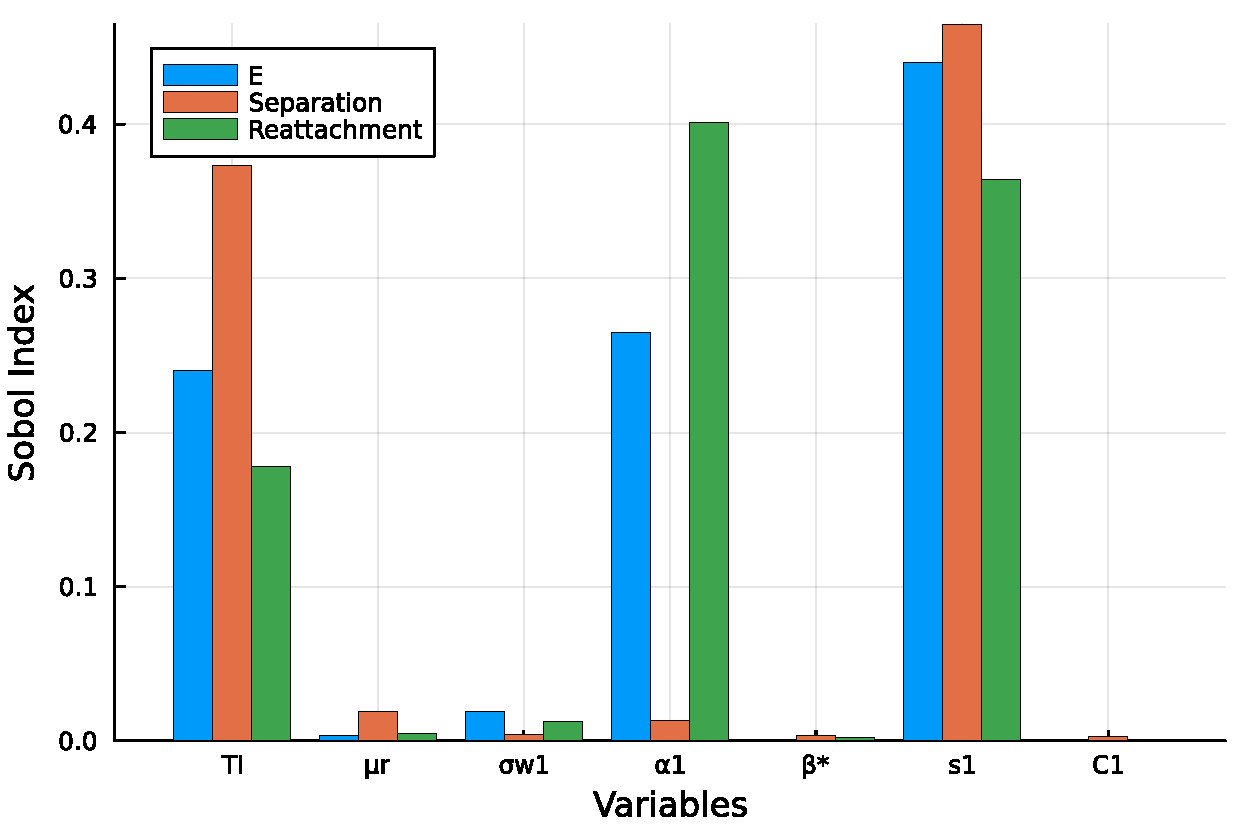
\includegraphics[width= 1\textwidth]{Figures/Sobol_sd7003.pdf}
			\begin{minipage}{0.95\textwidth}
			\vspace{0.1 cm}
			\justifying
			\noindent
			\scriptsize \textit{Sobol indexes for different parameters for SD7003 airfoil at Reynolds $\num{60000}$ at $\ang{4}$}
        \end{minipage}
}	

\headerbox{Industrial partner}{name=industrial,span=1,column=2,row=0, below=uq}{
Collaboration with \textit{STRATOS solution, Belgium}, for the in-flight test in the stratosphere.
  \hspace{0.01\textwidth}	
			\centering

\includegraphics[width= 0.95\textwidth]{Figures/STRATOS_black.png}
}		

\headerbox{}{name=references,column=2,below=industrial}{
\scriptsize										% Make the whole text 
\vspace{-0.4em} 										% Save some space at the beginning
\bibliographystyle{plain}							% Use plain style
\renewcommand{\section}[2]{\vskip 0.05em}		% Omit "References" title
          \renewcommand{\refname}{\vspace{-0.8em}}
          \bibliography{Library}
}
	
		
	\end{poster}
\end{document}